% Options for packages loaded elsewhere
% Options for packages loaded elsewhere
\PassOptionsToPackage{unicode}{hyperref}
\PassOptionsToPackage{hyphens}{url}
\PassOptionsToPackage{dvipsnames,svgnames,x11names}{xcolor}
%
\documentclass[
  spanish,
  a4paper,
  oneside]{scrbook}
\usepackage{xcolor}
\usepackage[top=25mm,bottom=25mm,left=30mm,right=20mm]{geometry}
\usepackage{amsmath,amssymb}
\setcounter{secnumdepth}{5}
\usepackage{iftex}
\ifPDFTeX
  \usepackage[T1]{fontenc}
  \usepackage[utf8]{inputenc}
  \usepackage{textcomp} % provide euro and other symbols
\else % if luatex or xetex
  \usepackage{unicode-math} % this also loads fontspec
  \defaultfontfeatures{Scale=MatchLowercase}
  \defaultfontfeatures[\rmfamily]{Ligatures=TeX,Scale=1}
\fi
\usepackage{lmodern}
\ifPDFTeX\else
  % xetex/luatex font selection
\fi
% Use upquote if available, for straight quotes in verbatim environments
\IfFileExists{upquote.sty}{\usepackage{upquote}}{}
\IfFileExists{microtype.sty}{% use microtype if available
  \usepackage[]{microtype}
  \UseMicrotypeSet[protrusion]{basicmath} % disable protrusion for tt fonts
}{}
\makeatletter
\@ifundefined{KOMAClassName}{% if non-KOMA class
  \IfFileExists{parskip.sty}{%
    \usepackage{parskip}
  }{% else
    \setlength{\parindent}{0pt}
    \setlength{\parskip}{6pt plus 2pt minus 1pt}}
}{% if KOMA class
  \KOMAoptions{parskip=half}}
\makeatother
% Make \paragraph and \subparagraph free-standing
\makeatletter
\ifx\paragraph\undefined\else
  \let\oldparagraph\paragraph
  \renewcommand{\paragraph}{
    \@ifstar
      \xxxParagraphStar
      \xxxParagraphNoStar
  }
  \newcommand{\xxxParagraphStar}[1]{\oldparagraph*{#1}\mbox{}}
  \newcommand{\xxxParagraphNoStar}[1]{\oldparagraph{#1}\mbox{}}
\fi
\ifx\subparagraph\undefined\else
  \let\oldsubparagraph\subparagraph
  \renewcommand{\subparagraph}{
    \@ifstar
      \xxxSubParagraphStar
      \xxxSubParagraphNoStar
  }
  \newcommand{\xxxSubParagraphStar}[1]{\oldsubparagraph*{#1}\mbox{}}
  \newcommand{\xxxSubParagraphNoStar}[1]{\oldsubparagraph{#1}\mbox{}}
\fi
\makeatother


\usepackage{longtable,booktabs,array}
\newcounter{none} % for unnumbered tables
\usepackage{calc} % for calculating minipage widths
% Correct order of tables after \paragraph or \subparagraph
\usepackage{etoolbox}
\makeatletter
\patchcmd\longtable{\par}{\if@noskipsec\mbox{}\fi\par}{}{}
\makeatother
% Allow footnotes in longtable head/foot
\IfFileExists{footnotehyper.sty}{\usepackage{footnotehyper}}{\usepackage{footnote}}
\makesavenoteenv{longtable}
\usepackage{graphicx}
\makeatletter
\newsavebox\pandoc@box
\newcommand*\pandocbounded[1]{% scales image to fit in text height/width
  \sbox\pandoc@box{#1}%
  \Gscale@div\@tempa{\textheight}{\dimexpr\ht\pandoc@box+\dp\pandoc@box\relax}%
  \Gscale@div\@tempb{\linewidth}{\wd\pandoc@box}%
  \ifdim\@tempb\p@<\@tempa\p@\let\@tempa\@tempb\fi% select the smaller of both
  \ifdim\@tempa\p@<\p@\scalebox{\@tempa}{\usebox\pandoc@box}%
  \else\usebox{\pandoc@box}%
  \fi%
}
% Set default figure placement to htbp
\def\fps@figure{htbp}
\makeatother


% definitions for citeproc citations
\NewDocumentCommand\citeproctext{}{}
\NewDocumentCommand\citeproc{mm}{%
  \begingroup\def\citeproctext{#2}\cite{#1}\endgroup}
\makeatletter
 % allow citations to break across lines
 \let\@cite@ofmt\@firstofone
 % avoid brackets around text for \cite:
 \def\@biblabel#1{}
 \def\@cite#1#2{{#1\if@tempswa , #2\fi}}
\makeatother
\newlength{\cslhangindent}
\setlength{\cslhangindent}{1.5em}
\newlength{\csllabelwidth}
\setlength{\csllabelwidth}{3em}
\newenvironment{CSLReferences}[2] % #1 hanging-indent, #2 entry-spacing
 {\begin{list}{}{%
  \setlength{\itemindent}{0pt}
  \setlength{\leftmargin}{0pt}
  \setlength{\parsep}{0pt}
  % turn on hanging indent if param 1 is 1
  \ifodd #1
   \setlength{\leftmargin}{\cslhangindent}
   \setlength{\itemindent}{-1\cslhangindent}
  \fi
  % set entry spacing
  \setlength{\itemsep}{#2\baselineskip}}}
 {\end{list}}
\usepackage{calc}
\newcommand{\CSLBlock}[1]{\hfill\break\parbox[t]{\linewidth}{\strut\ignorespaces#1\strut}}
\newcommand{\CSLLeftMargin}[1]{\parbox[t]{\csllabelwidth}{\strut#1\strut}}
\newcommand{\CSLRightInline}[1]{\parbox[t]{\linewidth - \csllabelwidth}{\strut#1\strut}}
\newcommand{\CSLIndent}[1]{\hspace{\cslhangindent}#1}

\ifLuaTeX
\usepackage[bidi=basic,shorthands=off]{babel}
\else
\usepackage[bidi=default,shorthands=off]{babel}
\fi
\ifLuaTeX
  \usepackage{selnolig} % disable illegal ligatures
\fi


\setlength{\emergencystretch}{3em} % prevent overfull lines

\providecommand{\tightlist}{%
  \setlength{\itemsep}{0pt}\setlength{\parskip}{0pt}}



 


\AtBeginDocument{\hypersetup{linkcolor=black}}
% ---------- Paquetes tipograficos y microajustes ----------
\usepackage{microtype}        % mejor interletrado y justificado
\usepackage{csquotes}         % comillas tipograficas
\usepackage{iftex}
\ifPDFTeX\else
  % Seleccion de fuentes solo cuando XeTeX/LuaTeX esta disponible.
  \IfFontExistsTF{TeX Gyre Termes}{
    \setmainfont{TeX Gyre Termes}
  }{
    \IfFontExistsTF{Latin Modern Roman}{\setmainfont{Latin Modern Roman}}{}
  }
  \IfFontExistsTF{TeX Gyre Heros}{
    \setsansfont{TeX Gyre Heros}
  }{
    \IfFontExistsTF{Latin Modern Sans}{\setsansfont{Latin Modern Sans}}{}
  }
  \IfFontExistsTF{TeX Gyre Cursor}{
    \setmonofont{TeX Gyre Cursor}
  }{
    \IfFontExistsTF{Latin Modern Mono}{\setmonofont{Latin Modern Mono}}{}
  }
\fi
\usepackage{enumitem}         % listas compactas
\setlist{itemsep=.2em, topsep=.2em}

% ---------- KOMA-Script: estilo de titulos y espaciado ----------
\KOMAoptions{
  headings=big,
  parskip=half,
  fontsize=12pt,
  appendixprefix=true
}
\setlength{\parindent}{1.5em}
\setlength{\parskip}{0.6em}
\usepackage{indentfirst}
\usepackage{setspace}         % Control del interlineado del documento
\setstretch{1.5}

% ---------- Encabezados y pies (scrlayer-scrpage) ----------
\usepackage[automark,headsepline]{scrlayer-scrpage}
\clearpairofpagestyles
\automark[chapter]{chapter}
\ihead{\pagemark}
\ohead{\itshape\headmark}
\setheadsepline{0.4pt}
\renewcommand*{\chaptermarkformat}{}
\renewcommand*{\chapterpagestyle}{scrheadings}
\pagestyle{scrheadings}
\makeatletter
\let\ps@plain\ps@scrheadings
\makeatother
\cfoot{}

% ---------- Hipervinculos mas sobrios ----------
\usepackage{hyperref}
\hypersetup{
  colorlinks=true,
  linkcolor=black,
  citecolor=[rgb]{0.05,0.2,0.5},
  urlcolor=[rgb]{0.05,0.2,0.5},
  pdfauthor={\@author},
  pdftitle={\@title}
}

% ---------- Leyendas de figuras/tablas ----------
\usepackage[labelfont=bf,textfont=it]{caption}
\captionsetup{
  skip=8pt
}

% ---------- Tabla de contenidos ----------
\KOMAoptions{toc=graduated}
\RedeclareSectionCommand[tocnumwidth=3em]{chapter}
\RedeclareSectionCommand[tocindent=3.25em,tocnumwidth=2.8em]{section}
\RedeclareSectionCommand[tocindent=6.5em,tocnumwidth=2.5em]{subsection}
\makeatletter
\newcommand*{\tocdotfill}{\leavevmode\leaders\hbox to .6em{\hss.\hss}\hfill}
\makeatother
\RedeclareSectionCommand[toclinefill=\tocdotfill]{chapter}
\RedeclareSectionCommand[toclinefill=\tocdotfill]{section}
\RedeclareSectionCommand[toclinefill=\tocdotfill]{subsection}
\renewcommand*{\contentsname}{Tabla de contenido}
\setkomafont{chapterentry}{\normalfont}
\setkomafont{chapterentrypagenumber}{\normalfont}

% ---------- Viudas/Huerfanas y cortes de pagina ----------
\clubpenalty=10000
\widowpenalty=10000
\displaywidowpenalty=10000

% ---------- Entorno abstract para scrbook ----------
\providecommand{\abstractname}{Resumen}
\makeatletter
\@ifundefined{abstract}{
  \newenvironment{abstract}{
    \cleardoublepage
    \thispagestyle{plain}
    \null\vfill
    \begin{center}
      {\bfseries\Large \abstractname\par}
    \end{center}\vspace{1em}
    \begingroup
  }{
    \par\endgroup
    \vfill\null
    \cleardoublepage
  }
}{}
\makeatother

% ---------- Soporte de subtitulo desde YAML ----------
\makeatletter
\providecommand{\subtitle}[1]{\gdef\@subtitle{#1}}
\providecommand{\@subtitle}{}
\makeatother

\makeatletter
\newcommand{\facso@iflist}[4]{%
  \begingroup
    \def\addvspace##1{}%
    \def\numberline##1{##1}%
    \def\facso@target{#2}%
    \newcount\facso@entrycount
    \facso@entrycount=0\relax
    \long\def\contentsline##1##2##3{%
      \def\facso@this{##1}%
      \ifx\facso@this\facso@target
        \advance\facso@entrycount\@ne
      \fi
    }%
    \InputIfFileExists{\jobname.#1}{}{}%
  \endgroup
  \ifnum\facso@entrycount>0\relax
    #3%
  \else
    #4%
  \fi}
\renewcommand{\listoffigures}{%
  \facso@iflist{lof}{figure}{%
    \cleardoublepage
    \phantomsection
    \addchap*{Listado de Figuras}%
    \thispagestyle{scrheadings}%
    \markboth{Listado de Figuras}{Listado de Figuras}%
    \addcontentsline{toc}{chapter}{Listado de Figuras}%
    \@starttoc{lof}%
    \cleardoublepage
    \automark[chapter]{chapter}%
  }{}}
\renewcommand{\listoftables}{%
  \facso@iflist{lot}{table}{%
    \cleardoublepage
    \phantomsection
    \addchap*{Listado de Tablas}%
    \thispagestyle{scrheadings}%
    \markboth{Listado de Tablas}{Listado de Tablas}%
    \addcontentsline{toc}{chapter}{Listado de Tablas}%
    \@starttoc{lot}%
    \cleardoublepage
    \automark[chapter]{chapter}%
  }{}}
\makeatother

% --- Desactivar portada y abstract automaticos de Pandoc (PDF) ---
\AtBeginDocument{\let\maketitle\relax}
\renewenvironment{abstract}{}{}
\providecommand{\appendixname}{}
\providecommand{\appendixtocname}{}
\providecommand{\appendixpagename}{}
\renewcommand*{\appendixname}{Anexo}
\renewcommand*{\appendixtocname}{Anexos}
\renewcommand*{\appendixpagename}{Anexos}
\usepackage{booktabs}
\usepackage{longtable}
\usepackage{array}
\usepackage{multirow}
\usepackage{wrapfig}
\usepackage{float}
\usepackage{colortbl}
\usepackage{pdflscape}
\usepackage{tabu}
\usepackage{threeparttable}
\usepackage{threeparttablex}
\usepackage[normalem]{ulem}
\usepackage{makecell}
\usepackage{xcolor}
\makeatletter
\@ifpackageloaded{bookmark}{}{\usepackage{bookmark}}
\makeatother
\makeatletter
\@ifpackageloaded{caption}{}{\usepackage{caption}}
\AtBeginDocument{%
\ifdefined\contentsname
  \renewcommand*\contentsname{Tabla de contenidos}
\else
  \newcommand\contentsname{Tabla de contenidos}
\fi
\ifdefined\listfigurename
  \renewcommand*\listfigurename{Listado de Figuras}
\else
  \newcommand\listfigurename{Listado de Figuras}
\fi
\ifdefined\listtablename
  \renewcommand*\listtablename{Listado de Tablas}
\else
  \newcommand\listtablename{Listado de Tablas}
\fi
\ifdefined\figurename
  \renewcommand*\figurename{Lista de figuras}
\else
  \newcommand\figurename{Lista de figuras}
\fi
\ifdefined\tablename
  \renewcommand*\tablename{Lista de tablas}
\else
  \newcommand\tablename{Lista de tablas}
\fi
}
\@ifpackageloaded{float}{}{\usepackage{float}}
\floatstyle{ruled}
\@ifundefined{c@chapter}{\newfloat{codelisting}{h}{lop}}{\newfloat{codelisting}{h}{lop}[chapter]}
\floatname{codelisting}{Listado}
\newcommand*\listoflistings{\listof{codelisting}{Listado de Listados}}
\makeatother
\makeatletter
\makeatother
\makeatletter
\@ifpackageloaded{caption}{}{\usepackage{caption}}
\@ifpackageloaded{subcaption}{}{\usepackage{subcaption}}
\makeatother
\usepackage{bookmark}
\IfFileExists{xurl.sty}{\usepackage{xurl}}{} % add URL line breaks if available
\urlstyle{same}
\hypersetup{
  pdftitle={Relación entre clase social subjetiva y percepción de delincuencia y corrupción en Chile},
  pdfauthor={Amaranta González; Amanda Rojo; Elena Yáñez},
  pdflang={es},
  colorlinks=true,
  linkcolor={Maroon},
  filecolor={Maroon},
  citecolor={Blue},
  urlcolor={Blue},
  pdfcreator={LaTeX via pandoc}}


\title{Relación entre clase social subjetiva y percepción de
delincuencia y corrupción en Chile}
\usepackage{etoolbox}
\makeatletter
\providecommand{\subtitle}[1]{% add subtitle to \maketitle
  \apptocmd{\@title}{\par {\large #1 \par}}{}{}
}
\makeatother
\subtitle{Trabajo final}
\author{Amaranta González \and Amanda Rojo \and Elena Yáñez}
\date{30 de junio de 2026}
\begin{document}
\frontmatter
\maketitle

% --- title-pdf.tex personalizado para portada formal ---
\makeatletter
\providecommand{\subtitle}[1]{\gdef\@subtitle{#1}}
\providecommand{\@subtitle}{}
\providecommand{\frontmattercontext}{}
\providecommand{\advisorname}{}
\providecommand{\advisorlabel}{FACSO}
\providecommand{\frontmatterlocation}{}
\InputIfFileExists{includes/cover-config.tex}{}{}

\newcommand{\PrintTitle}{%
  {\sffamily\bfseries\fontsize{24pt}{28pt}\selectfont \@title\par}%
}
\newcommand{\PrintSubtitle}{%
  \begingroup
  \edef\temp{\detokenize{\@subtitle}}%
  \ifx\temp\empty\relax
    % sin subtitulo
  \else
    {\sffamily\bfseries\large \@subtitle\par}%
  \fi
  \endgroup
}
\newcommand{\PrintAuthor}{%
  \begingroup
  \def\and{\\}% \and separa autores con salto de linea (en vez del \and de \maketitle estandar, que requiere una tabla abierta)
  {\Large\bfseries \@author\par}%
  \endgroup
}
\newcommand{\PrintDate}{%
  {\small \@date\par}%
}
\makeatother

\begin{titlepage}
\thispagestyle{empty}
\begin{center}
\vspace*{10mm}

% Logo o imagen institucional

\includegraphics[width=0.35\textwidth]{assets/cover.png}\par
\vspace{12mm}

% Titulo y subtitulo
\PrintTitle
\vspace{6mm}
\PrintSubtitle

\vspace{22mm}
\begingroup
\edef\temp{\detokenize{\frontmattercontext}}%
\ifx\temp\empty\relax
  % sin contexto adicional
\else
  {\normalsize \frontmattercontext\par}
\fi
\endgroup

\vspace{18mm}
\PrintAuthor

\vspace{16mm}
\begingroup
\edef\temp{\detokenize{\advisorname}}%
\ifx\temp\empty\relax
  % sin tutor
\else
  \rule{0.45\textwidth}{0.4pt}\par
  {\small \advisorlabel\ \advisorname\par}
\fi
\endgroup

\vfill
\begingroup
\edef\temp{\detokenize{\frontmatterlocation}}%
\ifx\temp\empty\relax
  % sin ubicacion
\else
  {\small \frontmatterlocation\par}
\fi
\endgroup
\PrintDate

\end{center}
\end{titlepage}

% Preliminares (numeros romanos) y estilo simple
\frontmatter
\pagestyle{scrheadings}

\setcounter{tocdepth}{2} % (o 1/3 segun prefieras)
\tableofcontents
\listoffigures
\listoftables


\mainmatter
\bookmarksetup{startatroot}

\chapter{Relación entre clase social subjetiva y percepción de
delincuencia y corrupción en
Chile}\label{relaciuxf3n-entre-clase-social-subjetiva-y-percepciuxf3n-de-delincuencia-y-corrupciuxf3n-en-chile}

\small\textbf{Palabras clave:} Ciencia Social Abierta \normalsize

\bookmarksetup{startatroot}

\chapter*{Abstract}\label{abstract}
\addcontentsline{toc}{chapter}{Abstract}

\markboth{Abstract}{Abstract}

El presente documento es un informe de investigación que aborda la clase
social subjetiva y su relación con la percepción de la delincuencia y
corrupción en Chile, utilizando datos de Latinobarómetro 2024. El
estudio se constituye de 3 hipotesis principales: (1) la clase social
subjetiva incide en la percepción de la delincuencia y corrupción, (2)
esta relación varía según el tipo de delito considerado, y (3) existe
una correlación negativa entre la clase social subjetiva y la percepción
de inseguridad. La investigación se basa en un enfoque de ciencia social
abierta, aplicando prácticas como pre-registro, datos abiertos y
reproducibilidad. Los resultados obtenidos permiten comprender mejor
cómo las percepciones de la corrupción se relacionan con la posición
social autopercibida, ofreciendo información valiosa para el diseño de
políticas públicas y estrategias de comunicación más efectivas. El
preregistro de la investigación se encuentra disponible en el
\href{https://www.doi.org/10.17605/OSF.IO/9R4AN}{Repositorio OSF.}

\bookmarksetup{startatroot}

\chapter{Introducción}\label{introducciuxf3n}

\bookmarksetup{startatroot}

\chapter{Introducción}\label{introducciuxf3n-1}

En los últimos años, la inseguridad se ha convertido en una de las
principales preocupaciones en el entorno nacional chileno. Esto, a pesar
de que los estudios empíricos indiquen lo contrario en comparación con
otros países ubicados en América Latina, donde las tasas de criminalidad
y violencia son significativamente más altas. Esta contradicción se
vuelve pertinente de analizar, pues como señala Klein
(\citeproc{ref-ImpactoMediosComunicacion}{2010}), ``la ubicación de
Chile bajo el promedio latinoamericano ha sido una constante desde
mediados de los años noventa a la fecha'' {[}p.~6{]}. De este modo,
Chile pertenece objetivamente al grupo de los países más seguros de la
región, llegando a ser considerado incluso el más seguro de América
Latina.

Sin embargo, la preocupación en la sociedad chilena en torno a la
delincuencia y el temor a ser víctima de un delito se mantienen en
niveles elevados, superando en ocasiones el promedio regional
latinoamericano. De hecho, Klein
(\citeproc{ref-ImpactoMediosComunicacion}{2010}) constata que, para el
año 2007, ``con 30,2\% Chile supera por casi un 13\% el promedio
latinoamericano'' {[}p.~119{]} en la percepción de la delincuencia como
problema principal, una brecha que evidencia la profunda desconexión
entre los indicadores objetivos de seguridad y la percepción ciudadana
en Chile.

Esta desconexión ha sido abordada por diversas líneas de investigación.
Por un lado, estudios como el de Klein
(\citeproc{ref-ImpactoMediosComunicacion}{2010}) han demostrado que los
medios de comunicación, y en particular el consumo frecuente de
noticias, juegan un rol central en la construcción de la percepción de
inseguridad en Chile, ``considerando el paisaje mediático y sobre todo
las características de los contenidos noticieros, los cuales tienden a
sobre-representar el tema de la delincuencia'' {[}p.~184{]}.

Layera et~al.
(\citeproc{ref-layeraInseguridadPercibidaBarrios2020}{2020}) demostraron
que la percepción que las personas tienen de su propia posición social
influye más en su sensación de inseguridad que las condiciones objetivas
del barrio. Según los autores, el estatus subjetivo ``es una medida más
sensitiva que el capital económico {[}\ldots{]} que podría evaluar con
mayor precisión la influencia acumulada de la posición social y
vulnerabilidad'' {[}p.~9{]}. Por lo que se vuelve pertinente analizar la
clase social autopercibida y cómo podría considerarse un predictor clave
al medir la percepción de la delincuencia.

En este contexto, la presente investigación se propone explorar si la
clase social subjetiva incide en la percepción de la delincuencia y,
específicamente, si esta relación varía según el tipo de delito
considerado. Se plantea que las personas que se autoposicionan en clases
sociales más bajas tenderán a percibir con mayor intensidad los delitos
vinculados a la violencia y el narcotráfico, mientras que aquellas
ubicadas en clases sociales más altas tenderán a percibir con mayor
fuerza la corrupción y el fraude.

Por lo que las preguntas que guiarán la investigación serán:

\begin{enumerate}
\def\labelenumi{\arabic{enumi}.}
\item
  ¿Cómo se relaciona la autopercepción de clase social con la percepción
  de la delincuencia en Chile, y varía esta relación según el tipo de
  delito considerado?
\item
  ¿Existe una diferencia significativa en la percepción de la
  delincuencia entre personas de clases sociales subjetivas bajas,
  medias y altas?
\item
  ¿Existe una correlación negativa entre la clase social subjetiva y la
  percepción de la delincuencia, de modo que a mayor clase social, menor
  percepción de inseguridad?
\end{enumerate}

Con el principal objetivo de: Analizar la relación entre la clase social
subjetiva y la percepción de la delincuencia en Chile, diferenciando el
tipo de delito, a partir de los datos de la encuesta Latinobarómetro
2024 (\citeproc{ref-Latinobarometro2024}{\emph{Latinobarometro 2024},
s.~f.}).

La contribución esperada a nivel teórico es que este estudio contribuya
a la literatura sobre la diferenciación social del miedo al delito en
Chile, actualizando la evidencia con datos de Latinobarómetro 2024 y
profundizando en la distinción entre tipos de delito. Esperando
confirmar que la clase social subjetiva incide no solo en la intensidad
del miedo, sino también en su dirección hacia ciertos fenómenos
delictivos.

En el nivel metodológico, el trabajo aplica prácticas de ciencia abierta
tales como el uso de pre-registro, datos abiertos, y centrado en la
posibilidad de reproducibilidad dentro del ámbito de las ciencias
sociales.

Por último, a nivel práctico, los resultados podrán entregar
herramientas para el diseño de políticas de seguridad y comunicación que
consideren las percepciones diferenciadas por clase social, evitando
enfoques homogéneos que no responden a la realidad de los distintos
grupos.

El presente trabajo se organizará de la siguiente manera: en la sección
de antecedentes, se revisa la literatura sobre la relación entre clase
social y percepción de inseguridad, con énfasis en el caso chileno y el
rol de los medios de comunicación. Luego, en metodología, se detalla el
uso de datos abiertos (Latinobarómetro 2024), el protocolo de
investigación (estructura IPO), las variables consideradas y las
prácticas de ciencia abierta (OSF, pre-registro, Quarto Book).
Posteriormente, se presentan los resultados obtenidos del análisis
estadístico, seguidos de su discusión a la luz de la literatura
revisada. Finalmente, se exponen las conclusiones, las limitaciones del
estudio y las proyecciones para futuras investigaciones, junto con la
disponibilidad del Preprint y los materiales reproducibles.

\bookmarksetup{startatroot}

\chapter{Antecedentes}\label{antecedentes}

\bookmarksetup{startatroot}

\chapter{Antecedentes}\label{antecedentes-1}

El estudio de la percepción de inseguridad ha sido abordado desde
diversas perspectivas que coinciden en señalar su autonomía relativa
respecto de los indicadores objetivos de criminalidad. La tesis de Klein
(\citeproc{ref-ImpactoMediosComunicacion}{2010}) constituye uno de los
antecedentes más relevantes para esta investigación, ya que analiza el
impacto de los medios de comunicación en la percepción de seguridad en
Chile y América Latina utilizando datos de Latinobarómetro 2007.

Klein (\citeproc{ref-ImpactoMediosComunicacion}{2010}) en sus resultados
demuestra que, en Chile, el consumo de noticias tiene un impacto
negativo en la percepción de seguridad, incluso mayor que el hecho de
haber sido víctima de un delito, y que la confianza en los medios
también influye en esta percepción. Dentro de su marco teórico, sostiene
que los medios de comunicación no solo informan, sino que construyen una
realidad distorsionada al sobre-representar la violencia y el crimen, lo
que genera una visión de un ``mundo peligroso y hostil, lo que a su vez
llevaría a un aumento injustificado de la sensación de temor en las
personas'' {[}p.~14{]}.

Este hallazgo es particularmente relevante para el caso chileno, donde
la cobertura mediática de la delincuencia, caracterizada por ser
intensa, sensacionalista y centrada en la Región Metropolitana, instala
el tema en la agenda pública. Esto hace que la ciudadanía lo perciba
como un problema prioritario, incluso cuando los indicadores objetivos
no lo justifican. Así, la percepción de inseguridad en Chile no responde
únicamente a la criminalidad real, sino que está mediada por la
construcción mediática de la realidad.

En segundo lugar, la clase social se ha posicionado como un predictor
clave dentro de la percepción de inseguridad. Investigaciones en el
contexto nacional sugieren que el estatus subjetivo, entendido como la
posición que las personas creen ocupar en la jerarquía social, permite
``evaluar con mayor precisión la influencia acumulada de la posición
social y vulnerabilidad, es decir, asociarse negativamente con el miedo
al crimen y los sentimientos de inseguridad''
(\citeproc{ref-layeraInseguridadPercibidaBarrios2020}{Layera et~al.,
2020, p. 9}). Esto significa que las personas que se autoperciben en
posiciones socioeconómicamente más bajas tienden a experimentar mayores
niveles de temor.

Entre los mecanismos explicativos de esta relación destaca el modelo de
vulnerabilidad social, el cual sostiene que los grupos más
desaventajados presentan una mayor exposición a riesgos y menores
recursos para afrontarlos. En este sentido, se ha planteado que el
bienestar subjetivo es un factor crítico, pues ``parece ser mucho más
importante como predictor de inseguridad que el bienestar objetivo''
(\citeproc{ref-layeraInseguridadPercibidaBarrios2020}{Layera et~al.,
2020, p. 23}). Este modelo distingue entre la vulnerabilidad física y la
social (vinculada al nivel educativo y recursos económicos), las cuales
interactúan para explicar por qué ciertos grupos sociales expresan
mayores niveles de temor al delito.

Adicionalmente, el modelo de victimización postula que las personas que
han experimentado victimización directa o indirecta tienden a
desarrollar mayores niveles de miedo. Sin embargo, la evidencia muestra
que la victimización indirecta puede ser determinante, ya que ``en la
práctica, las experiencias de victimización indirecta permiten optimizar
considerablemente el ajuste del modelo'' explicativo del miedo al crimen
(\citeproc{ref-layeraInseguridadPercibidaBarrios2020}{Layera et~al.,
2020, p. 21}). Este mecanismo se conecta directamente con el rol de los
medios de comunicación. En el caso específico de Chile, se ha demostrado
que ``el impacto del «consumo de noticias» es incluso mayor al impacto
de «haber sido victimizado»; es decir, las noticias en Chile tienden a
tener una mayor influencia en la «percepción de la seguridad pública»
que la experiencia propia''
(\citeproc{ref-ImpactoMediosComunicacion}{Klein, 2010, p. 166}).

Por último, el modelo de desorden, conocido como las ``ventanas rotas'',
enfatiza que la percepción de incivilidades físicas y sociales, como la
presencia de basura, grafitis, viviendas abandonadas o consumo de
sustancias en el espacio público, contribuyen significativamente a la
sensación de inseguridad, independientemente de los niveles reales de
criminalidad (\citeproc{ref-garciaFrancescGuillenLasierra2025}{García,
2025}). Estos signos de desorden suelen registrarse con mayor frecuencia
en barrios de clases bajas o con alta concentración de pobreza, lo que
refuerza la relación entre posición social y percepción de inseguridad
al sugerir una ruptura en los autocontroles comunitarios y la unión
entre vecinos.

En conjunto, los antecedentes revisados permiten justificar la
pertinencia de la presente investigación. En primer lugar, la evidencia
empírica disponible (\citeproc{ref-ImpactoMediosComunicacion}{Klein,
2010}) demuestra que en Chile existe una desconexión entre la seguridad
objetiva y la percepción ciudadana de inseguridad, y que los medios de
comunicación juegan un rol central en la construcción de esta brecha. En
segundo lugar, la literatura teórica analizada mediante los enfoques de
vulnerabilidad social, victimización y desorden señala consistentemente
que la clase social es un predictor significativo del miedo al delito.
Esto se debe a que las personas de sectores más desfavorecidos suelen
estar más expuestas a entornos complejos, poseen menos recursos de
seguridad residencial y conviven con signos de desorden que alimentan el
temor de manera constante.

\bookmarksetup{startatroot}

\chapter{Hipótesis}\label{hipuxf3tesis}

Las hipotesis planteadas en este estudio se centran en la relación entre
la percepción de la delincuencia y la clase social subjetiva. Todas
fueron pre registradas en Open Science Framework (OSF) y se pueden
consultar \href{https://www.doi.org/10.17605/OSF.IO/9R4AN}{aquí.}

\subsection{Hipotesis de diferencias}\label{hipotesis-de-diferencias}

Se espera que exista una diferencia entre los promedios de percepción de
la delincuencia entre clases sociales subjetivas bajas, medias y altas.
H0 (nula): No existe una diferencia entre los promedios de percepción de
la delincuencia entre clases sociales subjetivas bajas y altas.

\subsection{Hipotesis direccional}\label{hipotesis-direccional}

Respecto al tipo de delincuencia percibida, se espera que las clases
sociales subjetivas bajas perciban más delincuencia común relacionada a
la violencia y el narcotrafico, mientras que las clases sociales
subjetivas altas perciban más delincuencia relacionada a la corrupción y
el fraude. H0 (nula): No existe una diferencia en el tipo de
delincuencia percibida entre clases sociales subjetivas bajas y altas.

\subsection{Hipotesis correlacional}\label{hipotesis-correlacional}

Se espera que exista una correlación negativa entre la percepción de la
delincuencia y la clase social subjetiva, es decir, a medida que aumenta
la clase social subjetiva, la percepción de la delincuencia disminuye.
H0 (nula): No existe una correlación entre la percepción de la
delincuencia y la clase social subjetiva.

\bookmarksetup{startatroot}

\chapter{Métodos}\label{muxe9todos}

\section{Datos}\label{datos}

Los datos utilizados en esta investigación provienen de la Encuesta
Latinobarómetro 2024, la cual es una encuesta de opinión pública que se
realiza anualmente en 18 países de América Latina. La encuesta recopila
información sobre diversos temas, incluyendo percepción de la
delincuencia, clase social subjetiva, percepciones de la democracia,
entre otros.

\section{Protocolo de
Investigación}\label{protocolo-de-investigaciuxf3n}

Para este estudio se utiliza el protocolo IPO (Input-Process-Output), el
cual permite estructurar la investigación de manera clara y organizada.
En la carpeta Input se encuentra información externa como la base de
datos original, la base procesada y la bibliografía. En la carpeta
Process se encuentran los scripts de análisis y procesamiento de datos,
mientras que en la carpeta Output se encuentran tablas, gráficos y
salidas del procesamiento.

\section{Variables}\label{variables}

Para este estudio, se seleccionaron las variables relacionadas con la
percepción de la delincuencia y la clase social subjetiva. Se
construirán dos escalas: una para medir la percepción de la delincuencia
y otra para medir la percepción de la corrupción.

Las variables seleccionadas son:

\subsection{Clase social subjetiva}\label{clase-social-subjetiva}

\begin{itemize}
\tightlist
\item
  \textbf{S2:} La gente algunas veces se describe a sí misma como
  perteneciendo a una clase social. ¿Ud. se describiría como
  perteneciendo a la clase\ldots?(1=Alta, 2=Media Alta, 3=Media, 4=Media
  Baja, 5=Baja).
\end{itemize}

La clase social subjetiva será recodificada en tres categorías: Clase
Baja, Clase Media y Clase Alta, para facilitar el análisis y la
interpretación de los resultados.

\subsection{Escala de percepción de la delincuencia
común}\label{escala-de-percepciuxf3n-de-la-delincuencia-comuxfan}

\begin{itemize}
\tightlist
\item
  \textbf{P49ST.A:} De la lista de problemas que le voy a leer, ¿Cree
  Ud. que han aumentado mucho o poco, han permanecido igual o han
  disminuido poco o mucho en los últimos doce meses? La delincuencia en
  general ha\ldots.(1.Aumentado mucho, 2. Aumentado poco, 3. Permanecido
  igual, 4. Disminuido poco, 5. Disminuido mucho).
\item
  \textbf{P49ST.B:} De la lista de problemas que le voy a leer, ¿Cree
  Ud. que han aumentado mucho o poco, han permanecido igual o han
  disminuido poco o mucho en los últimos doce meses? La drogadicción
  ha\ldots.(1.Aumentado mucho, 2. Aumentado poco, 3. Permanecido igual,
  4. Disminuido poco, 5. Disminuido mucho).
\item
  \textbf{P51ST:} ¿Con qué frecuencia se preocupa Ud. de que pueda
  llegar a ser víctima de un delito con violencia? (1.Todo o casi todo
  el tiempo, 2. Algunas veces, 3. Ocasionalmente, 4. Nunca).
\item
  \textbf{P52N:} ¿Cuán grave cree que es el problema del narcotráfico y
  crimen organizado en (PAÍS)? (1.Muy grave, 2. Bastante grave, 3. Poco
  grave, 4. Nada grave).
\item
  \textbf{P53N:} ¿Cuál de las siguientes frases está más cerca de su
  manera de pensar? (1. (PAÍS) le está ganando la batalla al
  narcotráfico y el crimen organizado, 2. (PAÍS) está perdiendo la
  batalla al narcotráfico y el crimen organizado, 3. No se puede ganarle
  al narcotráfico y el crimen organizado).
\end{itemize}

Las variables seleccionadas para la escala serán recodificadas e
invertidas para que los valores más altos representen una mayor
percepción de la delincuencia común, asociada a violencia y
narcotráfico. Luego los valores son normalizados para que estén en un
rango de 0 a 100, y finalmente se calcula el promedio de los valores
normalizados para obtener una escala de percepción de la delincuencia
común.

\subsection{Escala de percepción de
corrupción}\label{escala-de-percepciuxf3n-de-corrupciuxf3n}

\begin{itemize}
\tightlist
\item
  \textbf{P49ST.C:} De la lista de problemas que le voy a leer, ¿Cree
  Ud. que han aumentado mucho o poco, han permanecido igual o han
  disminuido poco o mucho en los últimos doce meses? La corrupción
  ha\ldots.(1.Aumentado mucho, 2. Aumentado poco, 3. Permanecido igual,
  4. Disminuido poco, 5. Disminuido mucho).
\item
  \textbf{P54N:} En una escala dónde ``00'' es ``Para nada corrupto'' y
  ``10'' ``Totalmente corrupto'', ¿cuán corrupto cree Ud que es (PAÍS)?
  (0-10).
\item
  \textbf{P55ST:} ¿Cuánto cree Ud. que se ha progresado en reducir la
  corrupción en las instituciones del Estado en estos últimos 2 años?
  (1. Mucho, 2. Algo, 3. Poco, 4. Nada).
\end{itemize}

Dado que las variables de esta escala siguen la lógica de mayor
percepción de corrupción = mayor valor, no es necesario invertir los
valores, sólo son transformados a numérico. Luego los valores son
normalizados para que estén en un rango de 0 a 100, y finalmente se
calcula el promedio de los valores normalizados para obtener una escala
de percepción de la corrupción.

\section{Métodos}\label{muxe9todos-1}

Respecto a las pruebas de hipótesis, se realizan las pruebas
estadísticas correspondientes para respaldar o refutar las hipótesis
planteadas. Para la hipotesis de diferencia de medias se utiliza una
prueba ANOVA dado que se comparan más de dos grupos, para la hipotesis
direccional se harán dos pruebas ANOVA independientes, una para la
percepción de la delincuencia y otra para la percepción de la
corrupción, y para la hipotesis correlacional se utiliza el coeficiente
de correlación de Pearson entre las variables clase subjetiva y la
escala de delincuencia común.

\bookmarksetup{startatroot}

\chapter{Resultados}\label{resultados}

\section{Hipotesis de diferencias}\label{hipotesis-de-diferencias-1}

Para la hipótesis de diferencias de medias, donde se espera que exista
una diferencia entre los promedios de percepción de la delincuencia
entre clases sociales subjetivas bajas, medias y altas, se realizó un
análisis ANOVA para comparar las medias de la escala de percepción de la
delincuencia común entre los diferentes grupos de clase social
subjetiva.

\begin{verbatim}
               Df Sum Sq Mean Sq F value Pr(>F)
clase_grupos    2    182   91.19   0.697  0.498
Residuals    1190 155587  130.75               
7 observations deleted due to missingness
\end{verbatim}

Los resultados indican que la clase social subjetiva no tiene un efecto
significativo en la percepción de la delincuencia común, ya que el valor
p es mayor a 0.05 (F(2, 1190) = 0.697, p = 0.498). Esto sugiere que no
hay diferencias significativas en la percepción de la delincuencia común
entre los diferentes grupos de clase social subjetiva, en consecuencia
se acepta la hipótesis nula.

\section{Hipotesis direccional}\label{hipotesis-direccional-1}

Para la hipótesis direccional, donde se espera que las clases sociales
subjetivas bajas perciban más delincuencia común relacionada a la
violencia y el narcotráfico, mientras que las clases sociales subjetivas
altas perciban más delincuencia relacionada a la corrupción y el fraude,
se realizaron dos análisis ANOVA independientes, uno para la escala de
percepción de la delincuencia común, que se muestra en la primera
hipotésis y otro para la escala de percepción de la corrupción.

\begin{verbatim}
               Df Sum Sq Mean Sq F value        Pr(>F)    
clase_grupos    2  11424    5712   18.93 0.00000000805 ***
Residuals    1190 359036     302                          
---
Signif. codes:  0 '***' 0.001 '**' 0.01 '*' 0.05 '.' 0.1 ' ' 1
7 observations deleted due to missingness
\end{verbatim}

Los resultados del análisis ANOVA para la escala de percepción de la
delincuencia común indican que no hay diferencias significativas entre
los grupos de clase social subjetiva (F(2, 1190) = 0.697, p = 0.498).
Por otro lado, los resultados del análisis ANOVA para la escala de
percepción de la corrupción indican que existen diferencias
significativas entre los grupos de clase social subjetiva y la
percepción de la corrupción.

\begin{verbatim}
  Tukey multiple comparisons of means
    95% family-wise confidence level

Fit: aov(formula = escala_corrupcion ~ clase_grupos, data = data)

$clase_grupos
                            diff       lwr        upr     p adj
Clase Baja-Clase Alta  16.495609 10.092588 22.8986304 0.0000000
Clase Media-Clase Alta 14.035878  7.681955 20.3898004 0.0000008
Clase Media-Clase Baja -2.459731 -4.878616 -0.0408469 0.0452095
\end{verbatim}

Para verificar entre qué grupos existen diferencias significativas, se
realizó la prueba post-hoc de Tukey. Se encuentra que la clase baja
puntúa 16.5 puntos más alto que la clase alta en la escala de percepción
de la corrupción, la clase media puntúa 14.04 puntos más alto que la
clase alta y la clase media puntúa 2.46 puntos más bajo que la clase
baja. Estos resultados son significativos y sugieren que las clases
sociales subjetivas bajas y medias perciben más corrupción que las
clases sociales subjetivas altas.

\pandocbounded{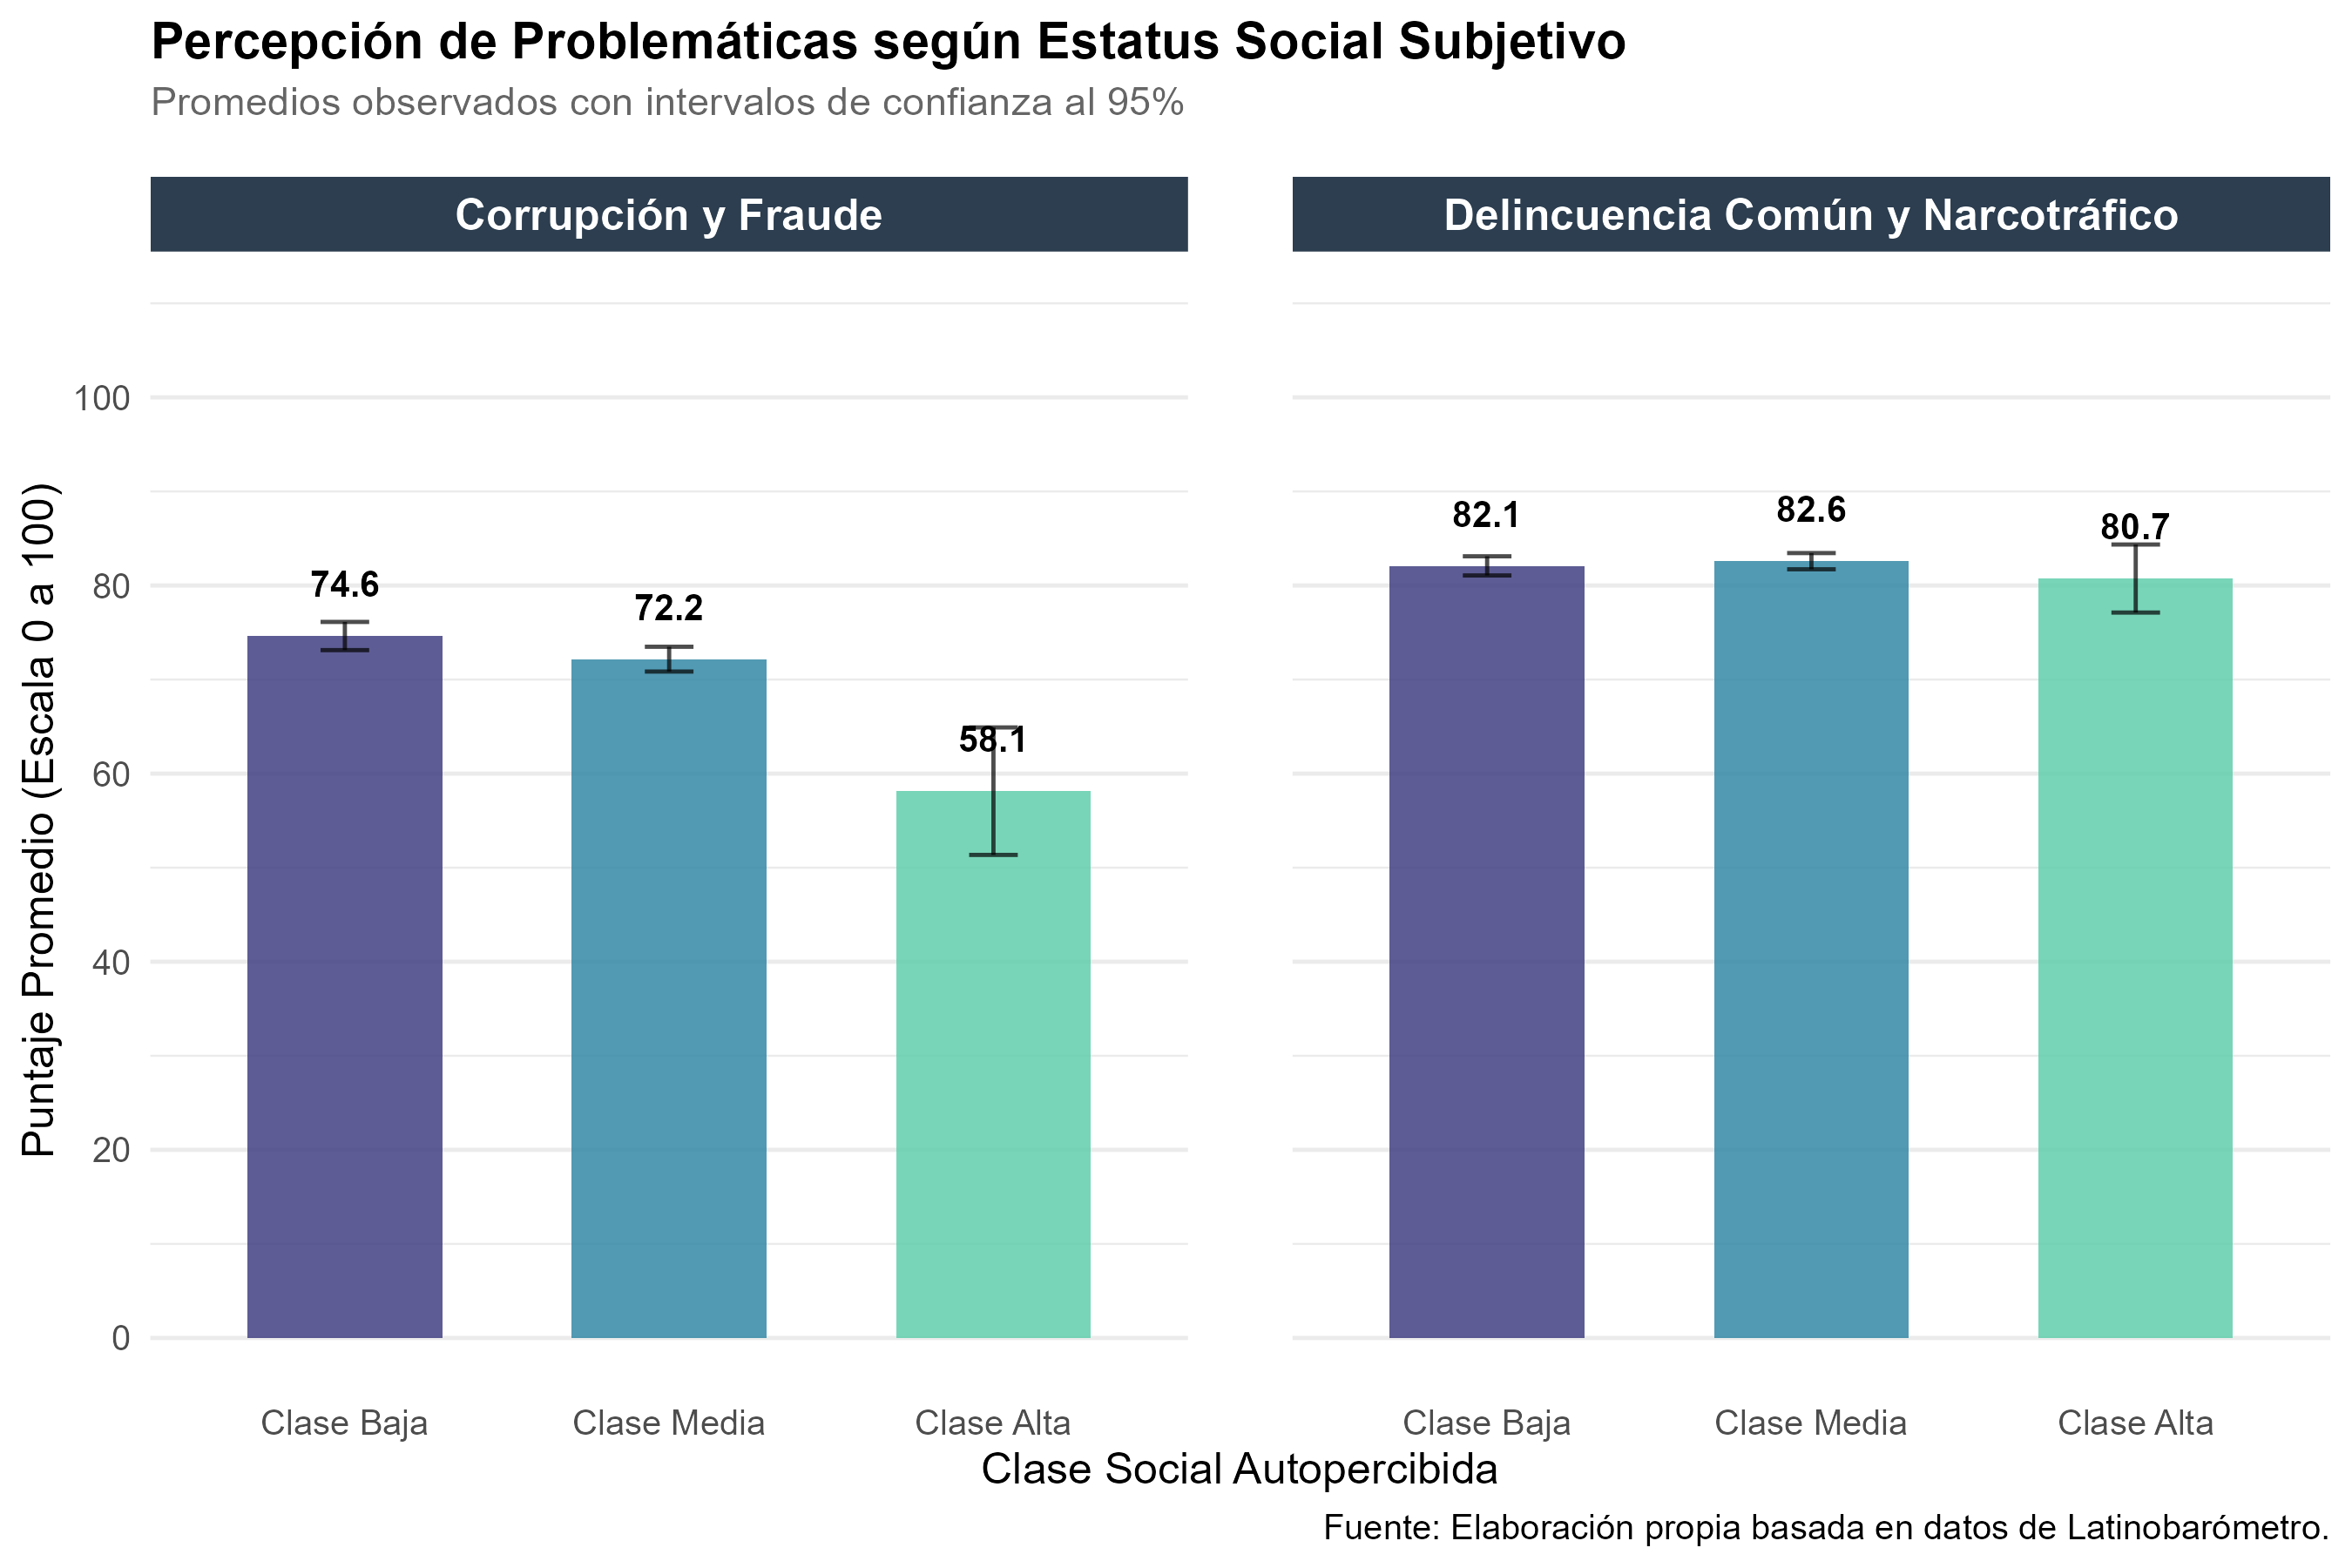
\includegraphics[keepaspectratio]{output/grafico-hipotesis2.png}}

\section{Hipotesis correlacional}\label{hipotesis-correlacional-1}

Para evaluar la hipotesis correlacional, donde se espera que exista una
correlación negativa entre la percepción de la delincuencia y la clase
social subjetiva, se realizó un análisis de correlación de Spearman
entre la variable de clase social subjetiva y la escala de percepción de
la delincuencia común.

\begin{verbatim}

    Spearman's rank correlation rho

data:  data$clase_subjetiva and data$escala_delincuencia_comun
S = 284667894, p-value = 0.8378
alternative hypothesis: true rho is not equal to 0
sample estimates:
         rho 
-0.005932208 
\end{verbatim}

Los resultados demuestran una ausencia de relación significativa entre
la percepción de la delincuencia y la clase social subjetiva (rho =
-0.005, p = 0.83). Dado que el valor p es mayor a 0.05, se acepta la
hipótesis nula y se conncluye que la clase social subjetiva no está
asociada con la percepción de la delincuencia común.

\section{Interpretaciones}\label{interpretaciones}

Las hipotesis 1 y 3 no fueron confirmadas, ya que no se encontraron
diferencias significativas en la percepción de la delincuencia común
entre los diferentes grupos de clase social subjetiva, ni tampoco se
encontró una correlación significativa entre la percepción de la
delincuencia y la clase social subjetiva. Esto puede interpretarse como
que la percepción de la delincuencia común no está influenciada por la
clase social subjetiva, lo que sugiere que otros factores pueden estar
influyendo en la percepción de la delincuencia y que la preocupación por
la delincuencia común es transversal a todas las clases sociales
subjetivas.

La hipotesis 2 tampoco fue confirmada en su totalidad, ya que si bien se
encontraron diferencias significativas en la percepción de la corrupción
entre los diferentes grupos de clase social subjetiva, no se encontraron
diferencias significativas en la percepción de la delincuencia común. Se
encuentra que las clases sociales subjetivas bajas y medias perciben más
corrupción que las clases sociales subjetivas altas, lo que sugiere que
la percepción de la corrupción está influenciada por la clase social
subjetiva. Esto puede interpretarse de distintas maneras, por ejemplo,
que las clases sociales subjetivas bajas y medias tienen una mayor
exposición a situaciones de corrupción al ser quienes más utilizan los
servicios públicos y la corrupción produce un deterioro directo en
estos. De la misma forma, los sectores de clase alta pueden tener una
percepción más positiva de la corrupción al estar más alejados de los
servicios públicos y no verse afectados directamente por la corrupción.
Además, en la realidad chilena, la corrupción es un tema que afecta
personalmente a los sectores de clase baja y media, siendo estos quienes
presentan una mayor desconfianza hacia las instituciones públicas y
privadas.

\section{Limitaciones y aportes}\label{limitaciones-y-aportes}

Si bien los resultados obtenidos en este estudio no confirman todas las
hipótesis planteadas, es importante destacar que el análisis realizado
proporciona información valiosa sobre la relación entre la percepción de
la delincuencia, la corrupción y la clase social subjetiva. Algunas de
las principales limitaciones corresponden a la naturaleza transversal
del estudio, que no permite establecer relaciones de causalidad entre
las variables analizadas. Además, la percepción de la delincuencia y la
corrupción puede estar influenciada por factores externos, como los
medios de comunicación y la experiencia personal, que no fueron
considerados en este estudio. Como aporte, este estudio abre una
importante línea de investigación sobre la relación entre la percepción
de la corrupción y la clase social subjetiva, que puede ser explorada en
futuros estudios con un enfoque más amplio y considerando otros factores
que puedan influir en la percepción de la corrupción. Además, los
resultados obtenidos pueden ser utilizados para considerar políticas
públicas enfocadas a la reducción de la corrupción y a una mejor
percepción de la ciudadanía hacia las instituciones públicas y privadas,
especialmente en los sectores de clase baja y media, que son quienes más
perciben la corrupción y quienes más se ven afectados por ella.

\bookmarksetup{startatroot}

\chapter{Conclusiones}\label{conclusiones}

Nuestros resultados no se corresponden con la literatura revisada en los
antecedentes (como Méndez Layera et al., 2020), especificamente respecto
a la afirmacion de que las clases bajas sienten más temor por su
vulnerabilidad social y residencial. Según nuestros resultados, todas
las clases sociales tienen percepciones similares de la inseguiridad y
el crimen. Como hipótesis tentativa, esta homogeneidad podría estar
relacionada al rol amplificador de los medios de comunicación planteado
por Klein (2010), el cual podria haber contribuido a nivelar el temor en
el debate público chileno. Dado que este estudio presenta la limitación
metodológica de no haber controlado por el consumo medial o la
victimización directa e indirecta, se requieren futuras investigaciones
para evaluar formalmente la validez de estas hipótesis en el Chile
actual. Nuestro resultados noss llevan a sugerir que las politicas
públicas no debiesen limitarse exclusivamente al control policial o a
programas tradicionales de prevención del delito. Por el contrario, los
datos evidencian la necesidad de priorizar el fortalecimiento de la
probidad y la transparencia en la gestión pública, dado que los
servicios estatales constituyen un lugar donde los estratos
socioeconómicos bajos y medios experimentan de manera más directa los
efectos de la corrupción como una manifestación de desigualdades
estructurales.

\bookmarksetup{startatroot}

\chapter{Referencias}\label{referencias}

\protect\phantomsection\label{refs}
\begin{CSLReferences}{1}{0}
\bibitem[\citeproctext]{ref-garciaFrancescGuillenLasierra2025}
García, J. O. (2025). {Francesc Guillén Lasierra y Ricard Brotat Jubert,
Coords. 40 años de Ventanas Rotas. Luces y Sombras. Bosh Editor, 2023,
396 pp. ISBN: 979-84-19580-36-8}. \emph{Revista Española de
Investigación Criminológica}, \emph{23}(1), e1028-e1028.
\url{https://doi.org/10.46381/reic.v23i1.1028}

\bibitem[\citeproctext]{ref-ImpactoMediosComunicacion}
Klein. (2010). \emph{El Impacto de Los Medios de Comunicación de Masas
En La Percepción de La Seguridad Pública. Un Estudio Empírico Del Caso
Chileno En El Contexto Latinoamericano}.
https://repositorio.uchile.cl/handle/2250/105817.

\bibitem[\citeproctext]{ref-Latinobarometro2024}
\emph{Latinobarometro 2024}. (s.~f.).
https://www.latinobarometro.org/latinobarometro-2024\#LAT-2024-selected-country-header.

\bibitem[\citeproctext]{ref-layeraInseguridadPercibidaBarrios2020}
Layera, M. L. M., Otero, G., \& Perret, V. (2020). {Inseguridad
Percibida en los Barrios de Santiago de Chile: La Importancia del
Bienestar Subjetivo}. \emph{Dados}, \emph{63}, e20170036.
\url{https://doi.org/10.1590/001152582020200}

\end{CSLReferences}


\backmatter

% --- Cuerpo del libro (capítulos) en arábigos ---
\mainmatter
\pagestyle{scrheadings}

% --- (Opcional) Estilo del índice general ---
% \addtocontents{toc}{\protect\thispagestyle{plain}}


\end{document}
